\documentclass[../main.tex]{subfiles}

\begin{document}
\chapter{Backgrounds}
\label{ch:backgrounds}

Different branches of research were used to build upon this work.
These topics and how they are connected to my work
are explained in more detail in this chapter.

In \autoref{sec:information_retrieval},
I will describe the process of \emph{information retrieval systems}.

The notion of \emph{agents} is described in \autoref{sec:agents}.
Agents try to act as rational and goal-oriented decision-makers.
In comparison to classical computer algorithms,
agents observe, plan and act autonomously in order to complete a task.
I will explain the basic concept of an agent and list the most important types of agents.
Section~\ref{sec:language_modeling} deals with \emph{language modeling}
and the current developments of large language models (LLMs).
Building upon the attention-based transformer architecture, modern large language models (LLMs)
can handle complex tasks such as text generation.
Moreover, the natural language interface of LLMs can be used for tasks in other domains.
An example of such a domain is \emph{LLM-based agents}, explained in section~\ref{sec:llm_agents}.
The text generation ability of the LLM itself is not of interest here,
but rather using the internal knowledge of the model to generate a decision of an agent.
This section gives an introduction to proposed frameworks and ideas for LLM agents.

\section{Information Retrieval}
\label{sec:information_retrieval}
Retrieval of information is essential for humans.
Information can be anything, like things seen by the eye,
thoughts or an article from a book.
A broad definition of information retrieval from \cite{Manning2009} is:
\begin{quote}
    Information retrieval (IR) is finding material (usually documents)
    of an unstructured nature (usually text)
    that satisfies an information need
    from within large collections (usually stored on computers).
\end{quote}
Modern information retrieval systems extend this definition with a step
dealing with the presentation of the information to the user.

Retrieving the best documents for a query from a large database
filled with information of different kinds is a classic problem in computer science.
There has been extensive research on database architectures and indexing algorithms.
Popular applications of IR algorithms are search engines
that enable fast access to billions of documents on the internet.
Before retrieving information from an information retrieval system,
the data is preprocessed and stored.
Then a user query initiates a series of steps that can rewrite the query,
retrieve relevant documents,
re-rank the relevant documents and finally present the information to the user.

\subsection{Information Retrieval Steps}

\begin{figure}[t]
    \centering
    \begin{tikzpicture}[
            node distance=1.5cm,
            every node/.style={block}]
        \node (query) at (0,0) {Query};
        \node (rewrite) [right=of query] {Rewrite};
        \node (retrieve) [right=of rewrite] {Retrieve};
        \node (DB) [below=of retrieve] {Database};
        \node (docs) [left=of DB] {Documents};
        \node (rerank) [right=of retrieve] {Re-Rank};
        \node (present) [right=of rerank] {Present};

        \draw[->] (query) -- (rewrite);
        \draw[->] (rewrite) -- (retrieve);
        \draw[->] (DB) -- (retrieve);
        \draw[->] (docs) -- node[draw=none, above] {index} (DB);
        \draw[->] (retrieve) -- (rerank);
        \draw[->] (rerank) -- (present);
    \end{tikzpicture}
    \caption{Every information retrieval process starts with a user query.
        The database is then queried to retrieve relevant documents to the query.
        Before presenting an answer to the user, the retrieved documents are ranked by another relevance measure.}
    \label{fig:ir_steps}
\end{figure}
Information retrieval systems consist of multiple steps.
Typically, the user interacts with an information retrieval system
by writing out a query that describes the information need.
A problem with queries written by humans is that they are not optimized for the following steps of the retrieval system.
Human writing sentences can include spelling mistakes missing words or even wrong descriptions of information.
In IR systems researchers try to mitigate such problems with query rewriting.
A core query rewriting technique is to expand the query with more words to improve the retrieval accuracy.

To retrieve documents that correlate to the search query,
different algorithms and models have been proposed.
For a long time, functions like the BM25 \cite{Robertson2009}
were often used to retrieve the best matching documents from a corpus.
Term-based bag-of-words functions like BM25 rank documents based on word occurrences in every document.
With neural network approaches becoming more popular,
the focus has shifted toward mapping documents to high-dimensional vectors called embeddings.
A similarity matrix can then be used to calculate the distance between to embeddings corresponding to the query and a document.

After a set of relevant documents was retrieved with an efficient retrieval method,
the documents are re-ranked by their relevance.
This time the algorithms used for ranking the documents are specialized towards quality rather than efficiency.
In addition, the re-ranking phase can include task-specific ranking strategies to meet user demands.

In the last step, the information is presented to the user.
Large language models have become a popular method to create user-friendly responses from retrieved documents.

\subsection{Indexing}

Before documents can be retrieved from a database,
they have to be stored.
How documents are stored is a crucial part of creating an information retrieval system.
While some data sources are delivered in structured formats like JSON or XML,
academic texts are published in journals, articles or conference proceedings.
All of these mediums are distributed as PDFs which is an unstructured data format.
The PDF format does not save the content
A preprocessing step is required before storing the documents to extract information from unstructured formats.
There are different techniques to preprocess text before storing it.
With \emph{tokenization}, sentences are split up into words, phrases or symbols.
Words with little information such as articles and prepositions are removed from the word list.
The words are called \emph{stop words}.
Furthermore, a \emph{stemmer} can be used to group words that have the same stem.
All of these preprocessing steps help to capture the semantics of a text or sentence.


\subsection{Evaluation}

Information retrieval systems are generally evaluated by categorizing documents
as \emph{relevant} or \emph{non-relevant} concerning an information need of the user \cite{Manning2009}.
The \emph{gold standard} defines which documents are relevant and non-relevant.
One has to consider that the relevance decision is made according to an \emph{information need} and not the query.
This distinction shows,
that a clear information need has to be present in order to effectively evaluate an IR system.

Although information retrieval can be seen as a two-label classification problem,
it can not be evaluated with an accuracy measure
that is the fraction of correct classifications.
As almost all documents will be non-relevant for any given query,
the system could achieve high accuracy by simply classifying all documents
as non-relevant to the query.
For that reason, two measures are used to evaluate IR systems.
\begin{description}
    \item[Precision] is the fraction of retrieved documents that are relevant:
        \begin{equation}
            \text{Precision} = \frac{\text{\#relevant retrieved}}{\text{\#retrieved}}
        \end{equation}
    \item[Recall] is the fraction of relevant documents that are retrieved:
        \begin{equation}
            \text{Recall} = \frac{\text{\#relevant retrieved}}{\text{\#relevant}}
        \end{equation}
\end{description}
Having these two measures is helpful, as different tasks have different requirements.
While high precision might be more important for the average web surfer,
a professional researcher might be more interested in high recall.
With the two measures trading off against each other, the \emph{F Measure} combines
them into a single one.
Often written as $F_1$, the balanced version equally weights precision and recall:
\begin{equation}
    F_1 = \frac{2PR}{P+R}
\end{equation}
where $P$ is the precision and $R$ is the recall.
These measures are computed on unordered sets of documents.
For documents ranked by relevance,
the measures are calculated for sets containing the top $k$ documents for different $k$.

Other properties of IR systems can be measured.
The indexing and search speeds are important to enable effective usage of an IR system.
Another property is the degree of complexity allowed by the query language.
Nonetheless, the ultimate measure is the user utility.
Here, all dimensions of evaluation culminate into a single idea,
which makes this very hard to measure objectively.
Each user has different tastes and needs for an IR system.
The document relevance measurement is therefore a major simplification that can only
approximate the user utility of a system.

\section{Agents}
\label{sec:agents}
Rationality is viewed as a core component of intelligence.
In computer science, computational entities that act rationally are called agents.
What it means to act rational is, and will stay an open research question for a long time.
However, to use the notion of an agent in practical work a more concrete definition has emerged.
An agent is anything that can be viewed as perceiving its environment through sensors
and acting upon that environment through actuators \cite{Russel2022}.
A human perceives the world through eyes and can act with hands or speech,
a software can perceive and act through software interfaces.
Both examples can be called agents.

A key step when constructing an agent is to define the \emph{task environment}.
The task environment consists of a performance measure, the environment, the actuators and the sensors \cite{Russel2022}.
Environments can be physical but also purely virtual, we are then using a software agent.

\subsection{Agent Types}

An agent consists of an agent architecture and an agent program.
While the agent architecture makes perceptions and actions through sensors and actuators available,
the agent program implements the mapping from perceptions to actions.
Agent programs can be categorized into four basic types that almost all agents are based on \cite{Russel2022}.
What kind of agent is useful depends on the given task environment.

\begin{figure}[t]
    \centering
    \begin{tikzpicture}[
            outer sep=auto,
            bg/.style={block, inner sep=1em, label={[above]:#1}}
        ]

        \node[block] (agent) at (0,0) {Agent Program};
        \node[above=2ex of agent.north] (sensors) {Sensors};
        \node[below=2ex of agent.south](actuators) {Actuators};
        \coordinate[right=4cm of sensors] (sensors_origin);
        \coordinate[right=4cm of actuators] (actuators_target);
        \draw[->] (sensors) -- (agent);
        \draw[->] (agent) -- (actuators);
        \draw[->] (sensors_origin) -- node[above] {Percepts} (sensors);
        \draw[->] (actuators) -- node[above] {Actions} (actuators_target);

        \begin{scope}[on background layer]
            \node[bg={Agent Architecture}, fit={(sensors) (agent) (actuators)}] (arch) {};
            \node[bg={Environment}, fit={(sensors_origin) (actuators_target)}, minimum width=1.5cm] (env) {};
        \end{scope}
    \end{tikzpicture}
    \caption{An agent as defined in \autocite{Russel2022}.
        The agent program runs on the agent architecture.
        Agents perceive their environment through sensors and act upon it using actuators.
        The agent program continuously maps perceptions to action and defines the agent type.}
    \label{fig:agent_overview}
\end{figure}

\begin{description}
    \item[Simple reflex agents]
        Simple reflex agents are the simplest kind of agent.
        They choose actions based on the current perceptions looking at the perception history.
        This means that even a bit of unobservability can break the agent.
    \item[Model-based reflex agents]
        Model-based reflex agents deal with partially observable environments
        by keeping an internal state of the world.
        This internal state depends on the perception history.
        Modeling physical or mental states is a complex topic that is heavily researched.
    \item[Goal-based agents]
        In many cases, the perception history is not enough to choose the best action.
        To be able to do that a goal is required.
        Goal-based agents search for action sequences that end in a goal state.
        This process is called planning.
    \item[Utility-based agents]
        Even with a goal in mind, there are cases where more than one action sequence leads to the goal state.
        To decide which action to select, utility-based agents choose the action that maximizes the expected utility.
        The utility function of the agent should ideally match the performance measure of the task environment.
\end{description}

To improve the performance of an agent it \emph{has to learn}.
All agent types can be extended to learning agents.
For an agent, learning means modifying each component
such that it better aligns with feedback from a new critic component \autocite{Russel2022}.
As a result of these modifications, the agent performance improves.

\section{Language Modeling}
\label{sec:language_modeling}
Language modeling is an important research area of computer science.
In recent years, developments have significantly sped up with the introduction of deep learning into language modeling.
The transformer network \cite{Vaswani2017} has been the base for many advancements in recent years.
Deriving from the transformer network,
massively scaled-up pre-trained transformer models \autocite{Brown2020}
enabled a big leap in the capabilities of language processing models.


\subsection{Transformer Networks}
\label{subsec:transformer}

Using recurrent structures such as recurrent neural networks
and long short-term memory \cite{Chung2014}
was the dominant strategy in sequence modeling
before transformer networks \cite{Vaswani2017}.
Every sentence token was represented as a hidden state
that is a function of all previous hidden states.
While this approach has a reasonable motivation,
the sequential nature constrains computation speed for a single training example.
This limitation is especially hindering for longer sequences,
where batching the training data is only possible to a memory limit.
Attempts to minimize sequential computation included convolutional networks
that can be computed in parallel \cite{Gehring2017}.
For these models, however,
the number of operations required to relate two tokens
grows in the distance of their positions in the sequence.
Attention mechanisms allow modeling token relationships
independent of their distance in a sequence.

\begin{figure}[t]
    \centering
    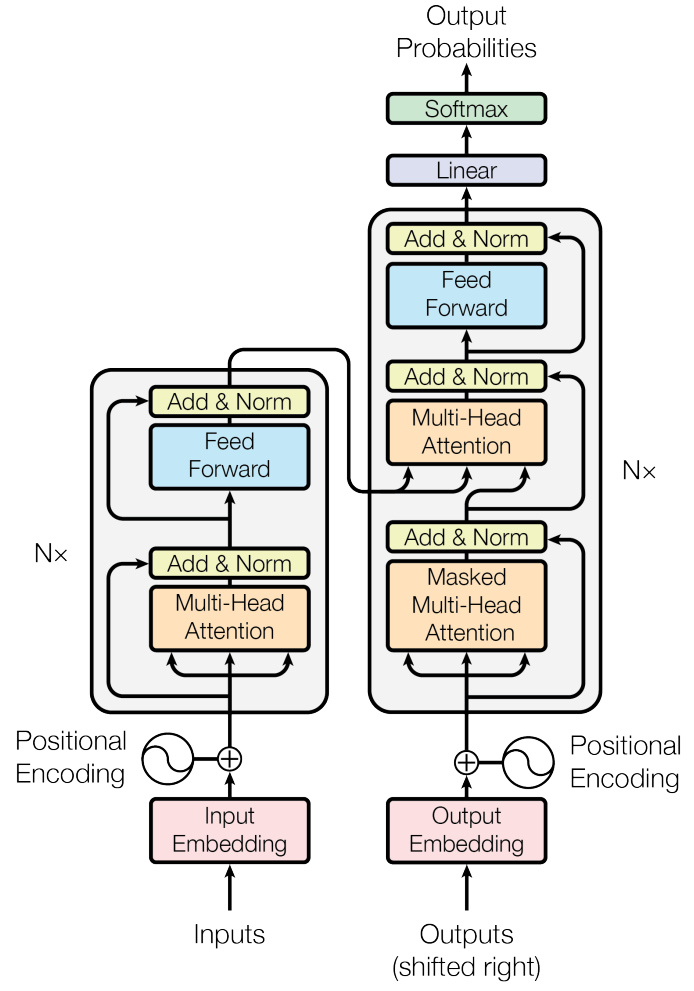
\includegraphics[scale=0.4]{include/images/transformer_architecture.png}
    \caption{
        The encoder-decoder architecture
        of a full transformer network \cite{Vaswani2017}.
        The encoder (left) can attend overall positions to learn rich embeddings.
        The decoder (right) can generate output sequences.
        The first decoder attention layer
        can only attend to previous positions of the input sequence,
        while the second can attend to the outputs of the encoder.
        This combines a sequence-to-sequence with
        autoregressive properties into the decoder.
    }
    \label{fig:transformer_arch}
\end{figure}

The transformer network \cite{Vaswani2017}
shown in \autoref{fig:transformer_arch}
was the first model that removed all recurrent structures
and only relies on attention mechanisms.
In particular,
they use multi-headed self-attention layers.
Attention mechanisms learn dependencies between tokens in sentences
without regard to their distance.
Their non-sequential characteristics allow for better parallelization.
Self-attention is an attention mechanism
that computes relations between different positions of the same sequence
to find a representation of the sequence.

Since the transformer architecture does not use any recurrent structures,
the order of the tokens in the sequence must be manually injected.
Positional encodings are added to the input embeddings to achieve this.

Like most language modeling networks,
a transformer consists of an encoder and a decoder.
The encoder has two sub-layers,
a multi-head attention block
and a fully connected feed-forward block.
The decoder is similar to the encoder
but has an additional multi-head attention layer
that attends to the outputs of the encoder.
The first attention layer is masked,
and the decoder input sequence is shifted to the right,
so only previous positions can be
attended by the decoder.

The full architecture has the capabilities of a classic sequence-to-sequence model
used for tasks like language translation.
All positions in the decoder can attend to all positions in the encoder.
For other tasks, however,
the individual encoder and decoder sections are a better fit,
as explained in the \autoref{subsec:embedding} and \autoref{subsec:gpt}.

\subsection{Generative Pre-Trained Transformers}
\label{subsec:gpt}

\begin{figure}[t]
    \centering
    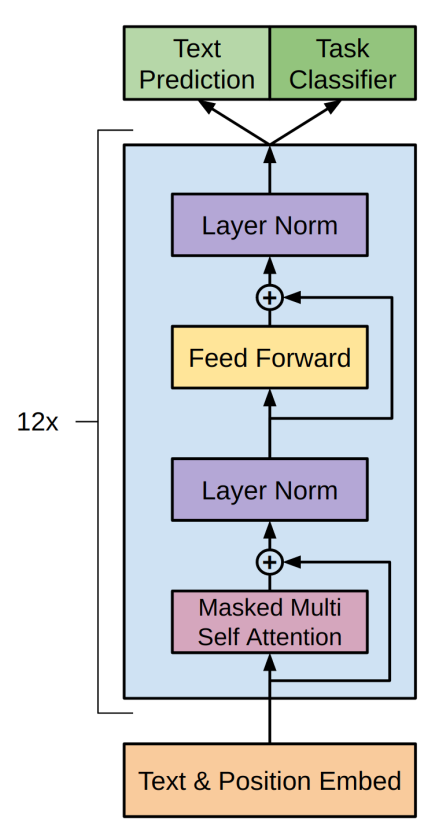
\includegraphics[scale=0.3]{include/images/gpt_architecture.png}
    \caption{
        The GPT architecture \cite{Radford2018}.
        A transformer encoder
        without connections to a previous encoder is used.
        The attention layer
        can only attend to previous positions in the input sequence.
        The decoder is stacked $12$ times before generating the final output.
    }
    \label{fig:gpt_arch}
\end{figure}


Decoder-only transformers are the base of generative pre-trained transformers (GPT).
The decoder used for GPT does not rely on the outputs of an encoder,
because it is designed for generation tasks.
In \autoref{fig:gpt_arch} we can see
that only the masked multi-head attention layer is kept in comparison to
the full transformer network.
The simple architecture enables faster pre-training and fine-tuning.

GPT is trained in two phases.
In the unsupervised pre-training phase,
the model is trained with big datasets of unlabeled text data.
The training objective here is
to accurately generate the next token of a sequence.

After the first pre-training phase,
the model needs to be fine-tuned for a specific task.
By including custom tokens in the fine-tuning dataset,
the decoder can learn to handle a variety of different tasks
such as text generation or classification.

Newer research on generation models focuses on scaling the network.
The \emph{scaling law} states
that by simply increasing the number of parameters of the network,
the model capabilities increase.
Furthermore,
after a certain level of scaling,
abilities emerge that the model was not directly trained on.

As large language models have reached parameter counts of over a billion,
only very few companies have the hardware to train or even run inference tasks.

\subsection{Embedding Models}
\label{subsec:embedding}

The left-to-right nature of the transformer encoder suits text generation tasks that only depend on previous tokens.
However, there are dependencies between tokens in both directions,
which means a decoder-only model can not capture all relations.

The amount of knowledge learned in the pre-training phase is encoded in embeddings.
Embeddings are high-dimensional vectors that represent a sequence of words or tokens.
Semantically similar documents are represented with embedding vectors that have a small distance,
while semantically different documents have a high distance.

BERT \cite{Devlin2019} uses the encoder part of a transformer network, to create rich embeddings of input sequences.
In pre-training, the bidirectional encoder is trained with two unsupervised tasks.
For the first task,
random tokens in the sequence are masked out to predict the masked tokens from the remaining tokens in the sequence.
In the second task, sentence-level relationships are learned by predicting the next sentence.
After pre-training, BERT can be fine-tuned on different downstream tasks
leveraging the rich bidirectional embeddings learned in pre-training.

\subsection{Instruction-Tuned Models}

Language models are trained to predict the next token of a sequence.
While a lot of knowledge is captured in the weights of the model,
most information on the internet is not formatted in a conversational style.
Because of this, language models need to be prompted in a specific way to be effective.
The prompt needs to be written such that its continuation yields the desired output.
This is not optimal for human users, as one would rather write in a conversational style.
The training objective of large language models is different from the objective
"follow the user's instructions helpfully and safely" \cite{Ouyang2022}.
Researchers say that the language model is not \emph{aligned}.
A popular attempt at aligning language models is reinforcement learning with human feedback (RLHF) \cite{Ouyang2022}.


Instruct models are fine-tuned versions of language models.
Capturing the intent of the user is a key challenge for language models.
This process is called \emph{alignment}.
A popular approach to the alignment problem is reinforcement learning with human feedback (RLHF) \cite{Ouyang2022}.
Handcrafted prompts are used to fine-tune GPT-3.
The outputs of the model are collected into a set and ranked by humans.
This set is then used to train a reward model.
With this reward model, the language model is further fine-tuned.
The resulting model is called \emph{InstructGPT} and performs better than the baseline GPT-3 model.

Large language models are trained to predict the next token of a sequence,
not to follow the instructions of the user.
This leads to some unwanted results such as toxic, harmful or fabricated answers that are not true.

\section{Large Language Model Agents}
\label{sec:llm_agents}
With the rise of large language models and their impressive capabilities in various language tasks,
efforts began to leverage them in agent systems.
Experiments to give GPT access to tools \autocite{Shen2023, Schick2023},
that large language models can use external functions
if they are prompted with a description of how to access them.

Four key reasons why large language models are suitable as agent brains are outlined in \cite{Xi2023}.
Agents should act autonomously without direct interventions from humans.
The generative capabilities and dynamically adjusted outputs based on the input fit that characteristic.

For practical applications, \autocite{Zhu2024} proposes a distinction between static and dynamic agents.
A static agent is characterized as a fixed pipeline that mimics the user behavior.
While this approach works,
it cannot deal with complex and sometimes random human actions.
The other type of agent can dynamically execute actions that are presented to it.
The most prominent way of using LLM for agents
is to build a prompt that contains all the information about the task,
and then ask it to propose the next action.
The prompt can contain descriptions of possible abilities, the task, guidelines,
information about the environment and more.

Experiments in \cite{Liu2023} showed
that large language models focus more on the first and last lines of the prompt
in their answer generation.
This needs to be respected when constructing long prompts to use LLMs for agents.

\subsection{LLM Agent Construction}

Most large language model agents follow a certain pattern
when implementing an agent with LLMs.
A construction framework for LLM agents consisting of four modules
is proposed in \cite{Wang2023}.
Their agent framework is composed of a profiling module, a memory module,
a planning module and an action module.

Before the actual execution of steps, an agent is given a profile that describes
the role of the agent.
This profile is usually written into the prompt that is sent to the language model.
Profiles can be handcrafted by simply adding a "You are an x" statement to the prompt.
Furthermore, profiles can be generated by LLMs which saves time for multiple agents
but does not allow for precise control in the profile crafting process.

Information is stored in the memory module.
Memory is used to keep a mental state of the environment and store new observations.
LLM agent memory types draw inspiration from human short-term and long-term memories.
Short-term memory is generally represented by the in-context information given in the language model prompt.
It is restricted by the context window length of the transformer architecture.
Long-term memory represents an external storage of information.
For LLM agents, a popular choice is a vector database,
that allows for quick query and retrieval of information.

Planning strategies for agents can be separated into planning with feedback
and without feedback.
Planning without feedback uses single-path or multi-path reasoning.
Techniques like Chain of Thought (CoT) and Zero-shot-CoT prompt LLMs
to "think step by step" \cite{Wei2022}.
This produces a step-by-step solution to a task that can be used as a plan
for the agent.
Other single-path reasoning approaches like HuggingGPT
prompt the language model after each reasoning step \cite{Shen2023}.
For multi-path reasoning CoT can be used again, now generating multiple plans
in a tree-like structure \cite{Yao2023}.
For complex tasks, the agent should be able to incorporate feedback into
the planning process.
The feedback can come from the environment, humans or from a feedback model.
All of these changes have to be represented in the language model prompt.

To act out the agents' decisions in the environment, the agent needs an
action module.
There are two main strategies for acting out actions.
For the first strategy,
the agent uses the task and the memory as prompts
to choose the next action in a continuous loop.
As the agent proceeds the memory builds up with the action history.
This allows for dynamic action choices while the agent is running.
The second strategy uses the task to create a fixed action plan
that is then executed strictly.
Here, the agent can not adapt dynamically.
The agent space defines the set of possible actions that can be performed.
Agents can leverage external tools and internal knowledge.
Types of external tools can include APIs, databases or other models
that specialize in a specific task.
The internal knowledge of a language model is also important for the action module.
When deciding which action should be used in a step,
The planning, conversation and commonsense understanding capabilities
are crucial to make a good decision.
The outcomes of actions can change the environment, the internal state and
also trigger new actions.

For LLM agents we do not have all the components of a classical agent
that were listed in the previous section about agent types.
\autocite{SignificantGravitas2024}

\subsection{Evaluation}

- subjective evaluation
- human annotation
- turing test
- objective evaluation

\end{document}
